\documentclass[1p]{elsarticle_modified}
%\bibliographystyle{elsarticle-num}

%\usepackage[colorlinks]{hyperref}
%\usepackage{abbrmath_seonhwa} %\Abb, \Ascr, \Acal ,\Abf, \Afrak
\usepackage{amsfonts}
\usepackage{amssymb}
\usepackage{amsmath}
\usepackage{amsthm}
\usepackage{scalefnt}
\usepackage{amsbsy}
\usepackage{kotex}
\usepackage{caption}
\usepackage{subfig}
\usepackage{color}
\usepackage{graphicx}
\usepackage{xcolor} %% white, black, red, green, blue, cyan, magenta, yellow
\usepackage{float}
\usepackage{setspace}
\usepackage{hyperref}

\usepackage{tikz}
\usetikzlibrary{arrows}

\usepackage{multirow}
\usepackage{array} % fixed length table
\usepackage{hhline}

%%%%%%%%%%%%%%%%%%%%%
\makeatletter
\renewcommand*\env@matrix[1][\arraystretch]{%
	\edef\arraystretch{#1}%
	\hskip -\arraycolsep
	\let\@ifnextchar\new@ifnextchar
	\array{*\c@MaxMatrixCols c}}
\makeatother %https://tex.stackexchange.com/questions/14071/how-can-i-increase-the-line-spacing-in-a-matrix
%%%%%%%%%%%%%%%

\usepackage[normalem]{ulem}

\newcommand{\msout}[1]{\ifmmode\text{\sout{\ensuremath{#1}}}\else\sout{#1}\fi}
%SOURCE: \msout is \stkout macro in https://tex.stackexchange.com/questions/20609/strikeout-in-math-mode

\newcommand{\cancel}[1]{
	\ifmmode
	{\color{red}\msout{#1}}
	\else
	{\color{red}\sout{#1}}
	\fi
}

\newcommand{\add}[1]{
	{\color{blue}\uwave{#1}}
}

\newcommand{\replace}[2]{
	\ifmmode
	{\color{red}\msout{#1}}{\color{blue}\uwave{#2}}
	\else
	{\color{red}\sout{#1}}{\color{blue}\uwave{#2}}
	\fi
}

\newcommand{\Sol}{\mathcal{S}} %segment
\newcommand{\D}{D} %diagram
\newcommand{\A}{\mathcal{A}} %arc


%%%%%%%%%%%%%%%%%%%%%%%%%%%%%5 test

\def\sl{\operatorname{\textup{SL}}(2,\Cbb)}
\def\psl{\operatorname{\textup{PSL}}(2,\Cbb)}
\def\quan{\mkern 1mu \triangleright \mkern 1mu}

\theoremstyle{definition}
\newtheorem{thm}{Theorem}[section]
\newtheorem{prop}[thm]{Proposition}
\newtheorem{lem}[thm]{Lemma}
\newtheorem{ques}[thm]{Question}
\newtheorem{cor}[thm]{Corollary}
\newtheorem{defn}[thm]{Definition}
\newtheorem{exam}[thm]{Example}
\newtheorem{rmk}[thm]{Remark}
\newtheorem{alg}[thm]{Algorithm}

\newcommand{\I}{\sqrt{-1}}
\begin{document}

%\begin{frontmatter}
%
%\title{Boundary parabolic representations of knots up to 8 crossings}
%
%%% Group authors per affiliation:
%\author{Yunhi Cho} 
%\address{Department of Mathematics, University of Seoul, Seoul, Korea}
%\ead{yhcho@uos.ac.kr}
%
%
%\author{Seonhwa Kim} %\fnref{s_kim}}
%\address{Center for Geometry and Physics, Institute for Basic Science, Pohang, 37673, Korea}
%\ead{ryeona17@ibs.re.kr}
%
%\author{Hyuk Kim}
%\address{Department of Mathematical Sciences, Seoul National University, Seoul 08826, Korea}
%\ead{hyukkim@snu.ac.kr}
%
%\author{Seokbeom Yoon}
%\address{Department of Mathematical Sciences, Seoul National University, Seoul, 08826,  Korea}
%\ead{sbyoon15@snu.ac.kr}
%
%\begin{abstract}
%We find all boundary parabolic representation of knots up to 8 crossings.
%
%\end{abstract}
%\begin{keyword}
%    \MSC[2010] 57M25 
%\end{keyword}
%
%\end{frontmatter}

%\linenumbers
%\tableofcontents
%
\newcommand\colored[1]{\textcolor{white}{\rule[-0.35ex]{0.8em}{1.4ex}}\kern-0.8em\color{red} #1}%
%\newcommand\colored[1]{\textcolor{white}{ #1}\kern-2.17ex	\textcolor{white}{ #1}\kern-1.81ex	\textcolor{white}{ #1}\kern-2.15ex\color{red}#1	}

{\Large $\underline{12n_{0461}~(K12n_{0461})}$}

\setlength{\tabcolsep}{10pt}
\renewcommand{\arraystretch}{1.6}
\vspace{1cm}\begin{tabular}{m{100pt}>{\centering\arraybackslash}m{274pt}}
\multirow{5}{120pt}{
	\centering
	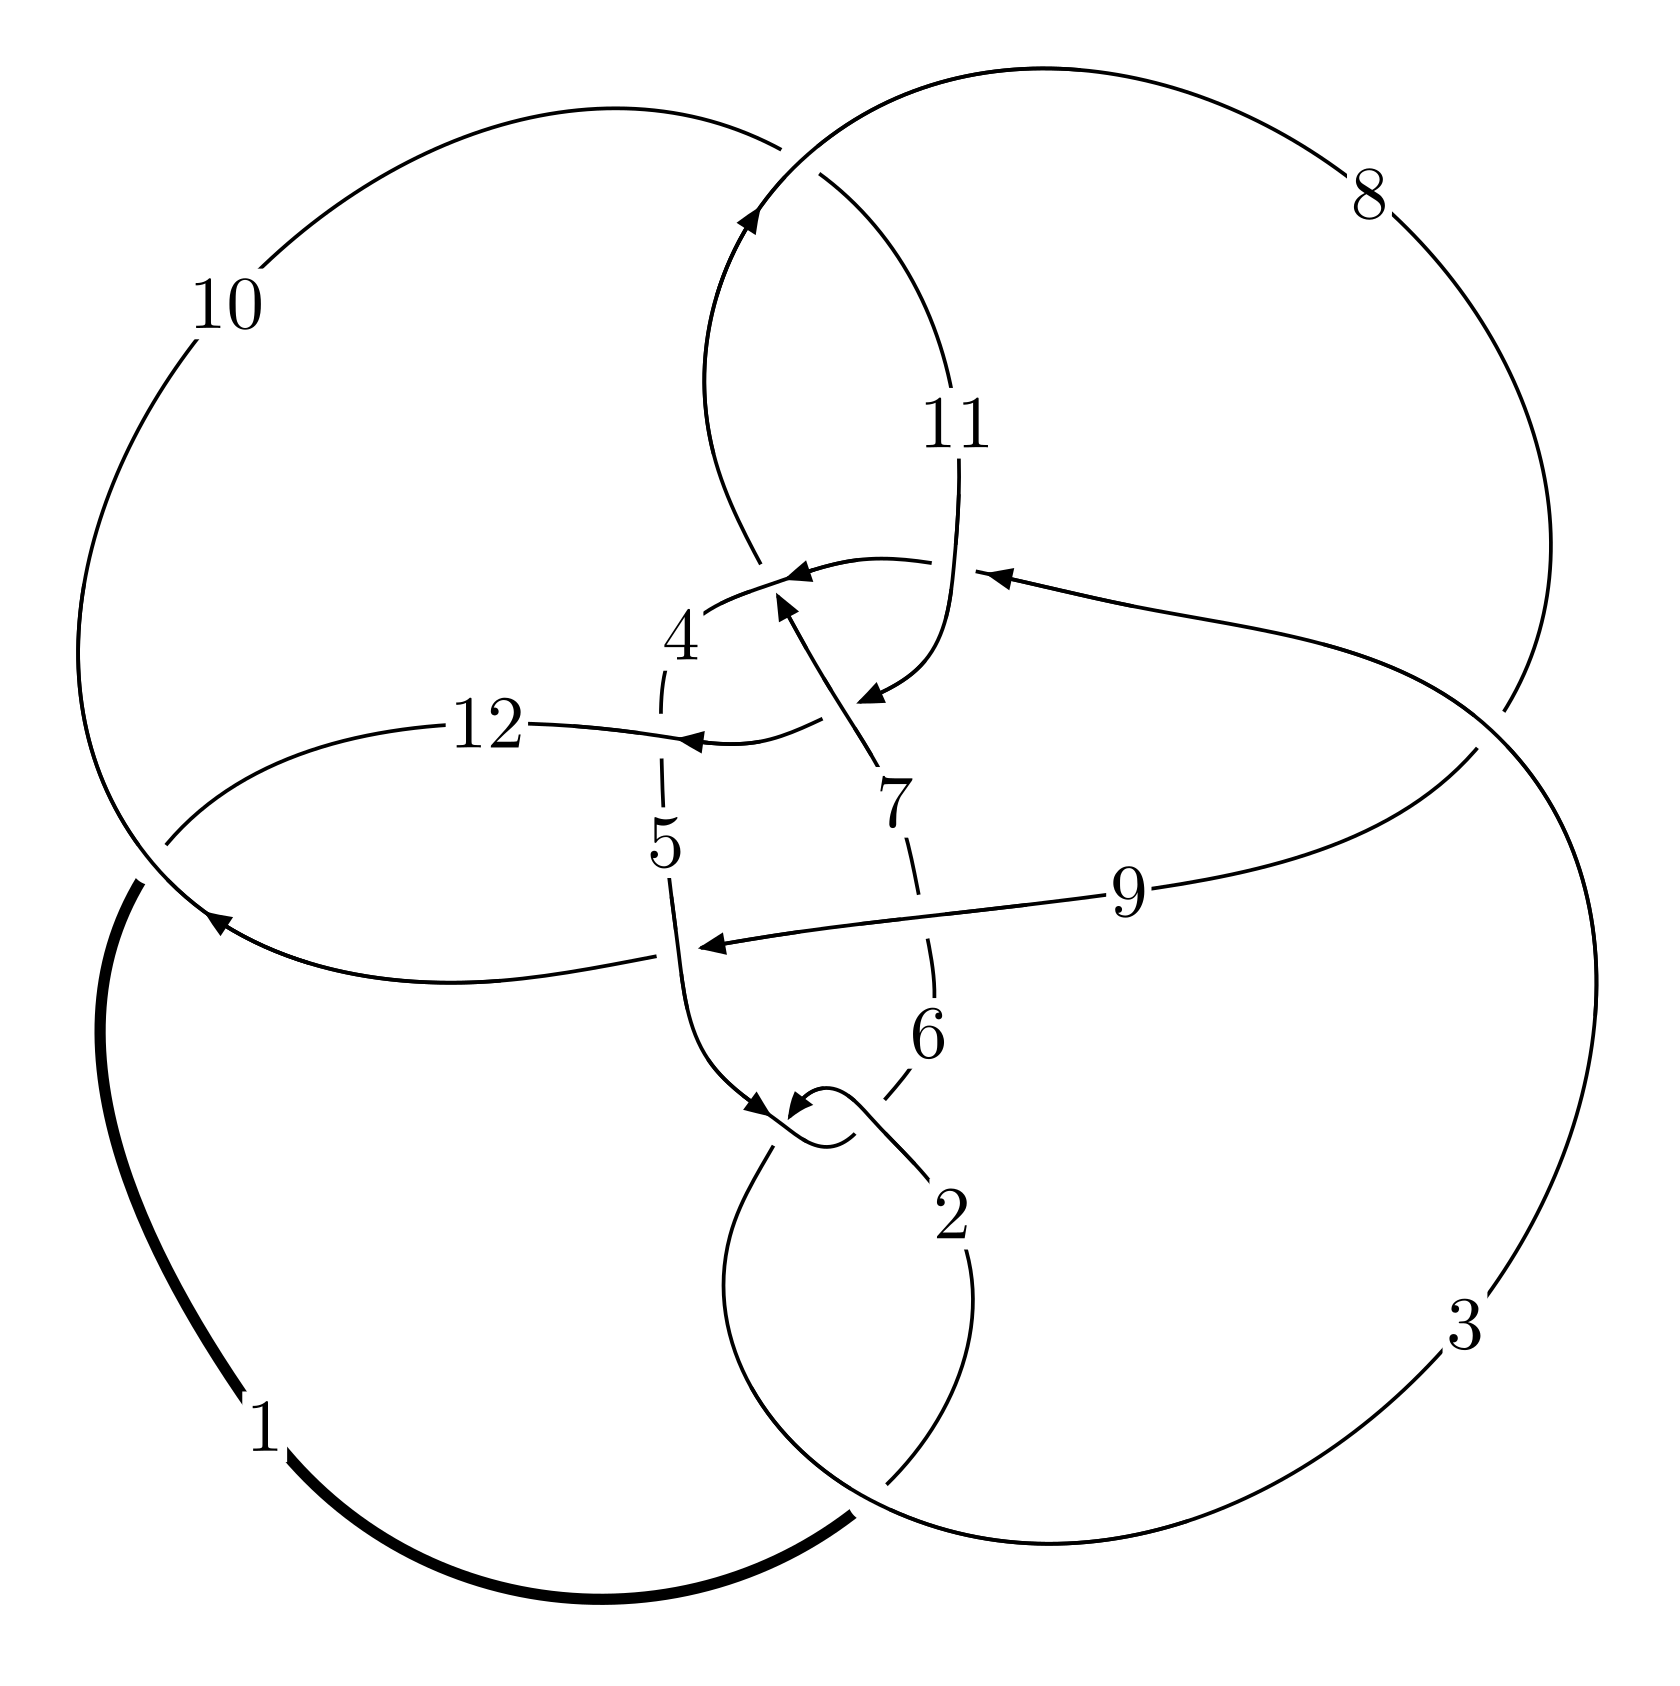
\includegraphics[width=112pt]{../../../GIT/diagram.site/Diagrams/png/2550_12n_0461.png}\\
\ \ \ A knot diagram\footnotemark}&
\allowdisplaybreaks
\textbf{Linearized knot diagam} \\
\cline{2-2}
 &
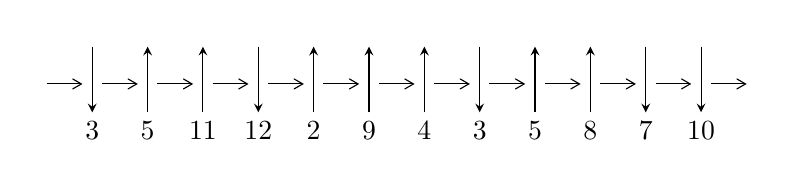
\begin{tikzpicture}[x=20pt, y=17pt]
	% nodes
	\node (C0) at (0, 0) {};
	\node (C1) at (1, 0) {};
	\node (C1U) at (1, +1) {};
	\node (C1D) at (1, -1) {3};

	\node (C2) at (2, 0) {};
	\node (C2U) at (2, +1) {};
	\node (C2D) at (2, -1) {5};

	\node (C3) at (3, 0) {};
	\node (C3U) at (3, +1) {};
	\node (C3D) at (3, -1) {11};

	\node (C4) at (4, 0) {};
	\node (C4U) at (4, +1) {};
	\node (C4D) at (4, -1) {12};

	\node (C5) at (5, 0) {};
	\node (C5U) at (5, +1) {};
	\node (C5D) at (5, -1) {2};

	\node (C6) at (6, 0) {};
	\node (C6U) at (6, +1) {};
	\node (C6D) at (6, -1) {9};

	\node (C7) at (7, 0) {};
	\node (C7U) at (7, +1) {};
	\node (C7D) at (7, -1) {4};

	\node (C8) at (8, 0) {};
	\node (C8U) at (8, +1) {};
	\node (C8D) at (8, -1) {3};

	\node (C9) at (9, 0) {};
	\node (C9U) at (9, +1) {};
	\node (C9D) at (9, -1) {5};

	\node (C10) at (10, 0) {};
	\node (C10U) at (10, +1) {};
	\node (C10D) at (10, -1) {8};

	\node (C11) at (11, 0) {};
	\node (C11U) at (11, +1) {};
	\node (C11D) at (11, -1) {7};

	\node (C12) at (12, 0) {};
	\node (C12U) at (12, +1) {};
	\node (C12D) at (12, -1) {10};
	\node (C13) at (13, 0) {};

	% arrows
	\draw[->,>={angle 60}]
	(C0) edge (C1) (C1) edge (C2) (C2) edge (C3) (C3) edge (C4) (C4) edge (C5) (C5) edge (C6) (C6) edge (C7) (C7) edge (C8) (C8) edge (C9) (C9) edge (C10) (C10) edge (C11) (C11) edge (C12) (C12) edge (C13) ;	\draw[->,>=stealth]
	(C1U) edge (C1D) (C2D) edge (C2U) (C3D) edge (C3U) (C4U) edge (C4D) (C5D) edge (C5U) (C6D) edge (C6U) (C7D) edge (C7U) (C8U) edge (C8D) (C9D) edge (C9U) (C10D) edge (C10U) (C11U) edge (C11D) (C12U) edge (C12D) ;
	\end{tikzpicture} \\
\hhline{~~} \\& 
\textbf{Solving Sequence} \\ \cline{2-2} 
 &
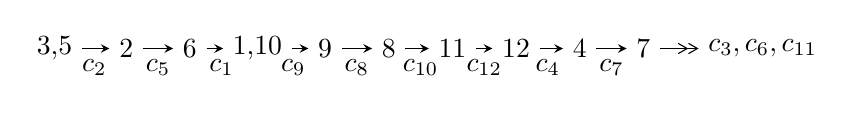
\begin{tikzpicture}[x=23pt, y=7pt]
	% node
	\node (A0) at (-1/8, 0) {3,5};
	\node (A1) at (1, 0) {2};
	\node (A2) at (2, 0) {6};
	\node (A3) at (49/16, 0) {1,10};
	\node (A4) at (33/8, 0) {9};
	\node (A5) at (41/8, 0) {8};
	\node (A6) at (49/8, 0) {11};
	\node (A7) at (57/8, 0) {12};
	\node (A8) at (65/8, 0) {4};
	\node (A9) at (73/8, 0) {7};
	\node (C1) at (1/2, -1) {$c_{2}$};
	\node (C2) at (3/2, -1) {$c_{5}$};
	\node (C3) at (5/2, -1) {$c_{1}$};
	\node (C4) at (29/8, -1) {$c_{9}$};
	\node (C5) at (37/8, -1) {$c_{8}$};
	\node (C6) at (45/8, -1) {$c_{10}$};
	\node (C7) at (53/8, -1) {$c_{12}$};
	\node (C8) at (61/8, -1) {$c_{4}$};
	\node (C9) at (69/8, -1) {$c_{7}$};
	\node (A10) at (11, 0) {$c_{3},c_{6},c_{11}$};

	% edge
	\draw[->,>=stealth]	
	(A0) edge (A1) (A1) edge (A2) (A2) edge (A3) (A3) edge (A4) (A4) edge (A5) (A5) edge (A6) (A6) edge (A7) (A7) edge (A8) (A8) edge (A9) ;
	\draw[->>,>={angle 60}]	
	(A9) edge (A10);
\end{tikzpicture} \\ 

\end{tabular} \\

\footnotetext{
The image of knot diagram is generated by the software ``\textbf{Draw programme}" developed by Andrew Bartholomew(\url{http://www.layer8.co.uk/maths/draw/index.htm\#Running-draw}), where we modified some parts for our purpose(\url{https://github.com/CATsTAILs/LinksPainter}).
}\phantom \\ \newline 
\centering \textbf{Ideals for irreducible components\footnotemark of $X_{\text{par}}$} 
 
\begin{align*}
I^u_{1}&=\langle 
1.96588\times10^{228} u^{66}+2.60681\times10^{228} u^{65}+\cdots+5.14418\times10^{229} b-5.03692\times10^{229},\\
\phantom{I^u_{1}}&\phantom{= \langle  }7.11870\times10^{230} u^{66}+1.26348\times10^{231} u^{65}+\cdots+1.59470\times10^{231} a+9.95544\times10^{232},\\
\phantom{I^u_{1}}&\phantom{= \langle  }u^{67}+2 u^{66}+\cdots+603 u+31\rangle \\
I^u_{2}&=\langle 
995343950102 u^{24}+3663166642595 u^{23}+\cdots+266559078319 b+2009076529451,\\
\phantom{I^u_{2}}&\phantom{= \langle  }-758722386667 u^{24}-2572820961963 u^{23}+\cdots+266559078319 a+2793047519965,\\
\phantom{I^u_{2}}&\phantom{= \langle  }u^{25}+3 u^{24}+\cdots+12 u+1\rangle \\
\\
\end{align*}
\raggedright * 2 irreducible components of $\dim_{\mathbb{C}}=0$, with total 92 representations.\\
\footnotetext{All coefficients of polynomials are rational numbers. But the coefficients are sometimes approximated in decimal forms when there is not enough margin.}
\newpage
\renewcommand{\arraystretch}{1}
\centering \section*{I. $I^u_{1}= \langle 1.97\times10^{228} u^{66}+2.61\times10^{228} u^{65}+\cdots+5.14\times10^{229} b-5.04\times10^{229},\;7.12\times10^{230} u^{66}+1.26\times10^{231} u^{65}+\cdots+1.59\times10^{231} a+9.96\times10^{232},\;u^{67}+2 u^{66}+\cdots+603 u+31 \rangle$}
\flushleft \textbf{(i) Arc colorings}\\
\begin{tabular}{m{7pt} m{180pt} m{7pt} m{180pt} }
\flushright $a_{3}=$&$\begin{pmatrix}1\\0\end{pmatrix}$ \\
\flushright $a_{5}=$&$\begin{pmatrix}0\\u\end{pmatrix}$ \\
\flushright $a_{2}=$&$\begin{pmatrix}1\\u^2\end{pmatrix}$ \\
\flushright $a_{6}=$&$\begin{pmatrix}u\\u^3+u\end{pmatrix}$ \\
\flushright $a_{1}=$&$\begin{pmatrix}u^2+1\\u^2\end{pmatrix}$ \\
\flushright $a_{10}=$&$\begin{pmatrix}-0.446398 u^{66}-0.792300 u^{65}+\cdots-931.788 u-62.4284\\-0.0382156 u^{66}-0.0506750 u^{65}+\cdots+6.93009 u+0.979148\end{pmatrix}$ \\
\flushright $a_{9}=$&$\begin{pmatrix}-0.446398 u^{66}-0.792300 u^{65}+\cdots-931.788 u-62.4284\\-0.0659120 u^{66}-0.0964250 u^{65}+\cdots-39.8309 u-2.13624\end{pmatrix}$ \\
\flushright $a_{8}=$&$\begin{pmatrix}-0.512310 u^{66}-0.888725 u^{65}+\cdots-971.619 u-64.5646\\-0.0659120 u^{66}-0.0964250 u^{65}+\cdots-39.8309 u-2.13624\end{pmatrix}$ \\
\flushright $a_{11}=$&$\begin{pmatrix}0.665717 u^{66}+1.16106 u^{65}+\cdots+1367.94 u+89.9273\\0.0771011 u^{66}+0.126191 u^{65}+\cdots+101.139 u+6.37264\end{pmatrix}$ \\
\flushright $a_{12}=$&$\begin{pmatrix}-0.0814414 u^{66}-0.0919983 u^{65}+\cdots+172.852 u+18.2940\\-0.105789 u^{66}-0.173936 u^{65}+\cdots-154.253 u-9.77732\end{pmatrix}$ \\
\flushright $a_{4}=$&$\begin{pmatrix}-0.146834 u^{66}-0.291150 u^{65}+\cdots-526.345 u-36.6710\\0.0133343 u^{66}+0.0148802 u^{65}+\cdots+9.89412 u+0.806420\end{pmatrix}$ \\
\flushright $a_{7}=$&$\begin{pmatrix}-0.782527 u^{66}-1.35663 u^{65}+\cdots-1584.69 u-109.331\\-0.142531 u^{66}-0.231198 u^{65}+\cdots-195.994 u-11.1014\end{pmatrix}$\\&\end{tabular}
\flushleft \textbf{(ii) Obstruction class $= -1$}\\~\\
\flushleft \textbf{(iii) Cusp Shapes $= 6.00516 u^{66}+10.3283 u^{65}+\cdots+10856.4 u+703.480$}\\~\\
\newpage\renewcommand{\arraystretch}{1}
\flushleft \textbf{(iv) u-Polynomials at the component}\newline \\
\begin{tabular}{m{50pt}|m{274pt}}
Crossings & \hspace{64pt}u-Polynomials at each crossing \\
\hline $$\begin{aligned}c_{1}\end{aligned}$$&$\begin{aligned}
&u^{67}+96 u^{66}+\cdots-6593 u-961
\end{aligned}$\\
\hline $$\begin{aligned}c_{2},c_{5}\end{aligned}$$&$\begin{aligned}
&u^{67}-2 u^{66}+\cdots+603 u-31
\end{aligned}$\\
\hline $$\begin{aligned}c_{3}\end{aligned}$$&$\begin{aligned}
&u^{67}-2 u^{65}+\cdots+12 u+1
\end{aligned}$\\
\hline $$\begin{aligned}c_{4}\end{aligned}$$&$\begin{aligned}
&u^{67}+u^{66}+\cdots+78 u-4
\end{aligned}$\\
\hline $$\begin{aligned}c_{6}\end{aligned}$$&$\begin{aligned}
&u^{67}-3 u^{66}+\cdots+1112592 u-190913
\end{aligned}$\\
\hline $$\begin{aligned}c_{7}\end{aligned}$$&$\begin{aligned}
&u^{67}-4 u^{66}+\cdots-152 u-19
\end{aligned}$\\
\hline $$\begin{aligned}c_{8}\end{aligned}$$&$\begin{aligned}
&u^{67}-21 u^{65}+\cdots+3707522 u-708772
\end{aligned}$\\
\hline $$\begin{aligned}c_{9}\end{aligned}$$&$\begin{aligned}
&u^{67}+u^{66}+\cdots-7924808 u-913579
\end{aligned}$\\
\hline $$\begin{aligned}c_{10}\end{aligned}$$&$\begin{aligned}
&u^{67}+10 u^{66}+\cdots-24 u-1
\end{aligned}$\\
\hline $$\begin{aligned}c_{11}\end{aligned}$$&$\begin{aligned}
&u^{67}+u^{66}+\cdots+22 u-1
\end{aligned}$\\
\hline $$\begin{aligned}c_{12}\end{aligned}$$&$\begin{aligned}
&u^{67}-5 u^{66}+\cdots+4917808 u-488737
\end{aligned}$\\
\hline
\end{tabular}\\~\\
\newpage\renewcommand{\arraystretch}{1}
\flushleft \textbf{(v) Riley Polynomials at the component}\newline \\
\begin{tabular}{m{50pt}|m{274pt}}
Crossings & \hspace{64pt}Riley Polynomials at each crossing \\
\hline $$\begin{aligned}c_{1}\end{aligned}$$&$\begin{aligned}
&y^{67}-248 y^{66}+\cdots+1205710659 y-923521
\end{aligned}$\\
\hline $$\begin{aligned}c_{2},c_{5}\end{aligned}$$&$\begin{aligned}
&y^{67}+96 y^{66}+\cdots-6593 y-961
\end{aligned}$\\
\hline $$\begin{aligned}c_{3}\end{aligned}$$&$\begin{aligned}
&y^{67}-4 y^{66}+\cdots+52 y-1
\end{aligned}$\\
\hline $$\begin{aligned}c_{4}\end{aligned}$$&$\begin{aligned}
&y^{67}-15 y^{66}+\cdots+2428 y-16
\end{aligned}$\\
\hline $$\begin{aligned}c_{6}\end{aligned}$$&$\begin{aligned}
&y^{67}+129 y^{66}+\cdots-167561891380 y-36447773569
\end{aligned}$\\
\hline $$\begin{aligned}c_{7}\end{aligned}$$&$\begin{aligned}
&y^{67}+6 y^{66}+\cdots-8740 y-361
\end{aligned}$\\
\hline $$\begin{aligned}c_{8}\end{aligned}$$&$\begin{aligned}
&y^{67}-42 y^{66}+\cdots+5030461829868 y-502357747984
\end{aligned}$\\
\hline $$\begin{aligned}c_{9}\end{aligned}$$&$\begin{aligned}
&y^{67}+99 y^{66}+\cdots+1331996748366 y-834626589241
\end{aligned}$\\
\hline $$\begin{aligned}c_{10}\end{aligned}$$&$\begin{aligned}
&y^{67}+18 y^{66}+\cdots-86 y-1
\end{aligned}$\\
\hline $$\begin{aligned}c_{11}\end{aligned}$$&$\begin{aligned}
&y^{67}+5 y^{66}+\cdots+12 y-1
\end{aligned}$\\
\hline $$\begin{aligned}c_{12}\end{aligned}$$&$\begin{aligned}
&y^{67}-111 y^{66}+\cdots+2732023039434 y-238863855169
\end{aligned}$\\
\hline
\end{tabular}\\~\\
\newpage\flushleft \textbf{(vi) Complex Volumes and Cusp Shapes}
$$\begin{array}{c|c|c}  
\text{Solutions to }I^u_{1}& \I (\text{vol} + \sqrt{-1}CS) & \text{Cusp shape}\\
 \hline 
\begin{aligned}
u &= \phantom{-}0.457533 + 0.954014 I \\
a &= \phantom{-}0.589994 + 0.995559 I \\
b &= \phantom{-}0.778600 + 0.667694 I\end{aligned}
 & -2.30669 - 1.69781 I & \phantom{-0.000000 } 0 \\ \hline\begin{aligned}
u &= \phantom{-}0.457533 - 0.954014 I \\
a &= \phantom{-}0.589994 - 0.995559 I \\
b &= \phantom{-}0.778600 - 0.667694 I\end{aligned}
 & -2.30669 + 1.69781 I & \phantom{-0.000000 } 0 \\ \hline\begin{aligned}
u &= -0.115958 + 1.054650 I \\
a &= \phantom{-}0.263031 + 0.627824 I \\
b &= \phantom{-}0.21100 + 1.58802 I\end{aligned}
 & -0.557773 - 1.254050 I & \phantom{-0.000000 } 0 \\ \hline\begin{aligned}
u &= -0.115958 - 1.054650 I \\
a &= \phantom{-}0.263031 - 0.627824 I \\
b &= \phantom{-}0.21100 - 1.58802 I\end{aligned}
 & -0.557773 + 1.254050 I & \phantom{-0.000000 } 0 \\ \hline\begin{aligned}
u &= -0.193472 + 0.917062 I \\
a &= -0.773951 + 0.955297 I \\
b &= \phantom{-}0.193510 + 0.352286 I\end{aligned}
 & -4.33901 - 2.24983 I & \phantom{-0.000000 } 0 \\ \hline\begin{aligned}
u &= -0.193472 - 0.917062 I \\
a &= -0.773951 - 0.955297 I \\
b &= \phantom{-}0.193510 - 0.352286 I\end{aligned}
 & -4.33901 + 2.24983 I & \phantom{-0.000000 } 0 \\ \hline\begin{aligned}
u &= \phantom{-}0.893939 + 0.275897 I \\
a &= -0.407031 - 0.202432 I \\
b &= -0.623251 + 0.431858 I\end{aligned}
 & \phantom{-}0.01989 - 3.98298 I & \phantom{-0.000000 } 0 \\ \hline\begin{aligned}
u &= \phantom{-}0.893939 - 0.275897 I \\
a &= -0.407031 + 0.202432 I \\
b &= -0.623251 - 0.431858 I\end{aligned}
 & \phantom{-}0.01989 + 3.98298 I & \phantom{-0.000000 } 0 \\ \hline\begin{aligned}
u &= -0.697295 + 0.620282 I \\
a &= -0.364005 + 0.741958 I \\
b &= -0.087737 - 1.325970 I\end{aligned}
 & -0.80774 + 6.08975 I & \phantom{-0.000000 } 0 \\ \hline\begin{aligned}
u &= -0.697295 - 0.620282 I \\
a &= -0.364005 - 0.741958 I \\
b &= -0.087737 + 1.325970 I\end{aligned}
 & -0.80774 - 6.08975 I & \phantom{-0.000000 } 0\\
 \hline 
 \end{array}$$\newpage$$\begin{array}{c|c|c}  
\text{Solutions to }I^u_{1}& \I (\text{vol} + \sqrt{-1}CS) & \text{Cusp shape}\\
 \hline 
\begin{aligned}
u &= \phantom{-}0.187614 + 0.909547 I \\
a &= \phantom{-}0.751918 + 1.020130 I \\
b &= \phantom{-}0.512623 - 0.137739 I\end{aligned}
 & -2.66802 - 2.88160 I & \phantom{-0.000000 } 0 \\ \hline\begin{aligned}
u &= \phantom{-}0.187614 - 0.909547 I \\
a &= \phantom{-}0.751918 - 1.020130 I \\
b &= \phantom{-}0.512623 + 0.137739 I\end{aligned}
 & -2.66802 + 2.88160 I & \phantom{-0.000000 } 0 \\ \hline\begin{aligned}
u &= -0.516210 + 0.989811 I \\
a &= \phantom{-}0.103606 + 0.654257 I \\
b &= \phantom{-}0.409249 + 0.491498 I\end{aligned}
 & -0.24728 - 2.81998 I & \phantom{-0.000000 } 0 \\ \hline\begin{aligned}
u &= -0.516210 - 0.989811 I \\
a &= \phantom{-}0.103606 - 0.654257 I \\
b &= \phantom{-}0.409249 - 0.491498 I\end{aligned}
 & -0.24728 + 2.81998 I & \phantom{-0.000000 } 0 \\ \hline\begin{aligned}
u &= \phantom{-}0.400784 + 1.045870 I \\
a &= -0.43114 - 1.47222 I \\
b &= \phantom{-}0.155940 - 0.982519 I\end{aligned}
 & -3.41227 - 6.93248 I & \phantom{-0.000000 } 0 \\ \hline\begin{aligned}
u &= \phantom{-}0.400784 - 1.045870 I \\
a &= -0.43114 + 1.47222 I \\
b &= \phantom{-}0.155940 + 0.982519 I\end{aligned}
 & -3.41227 + 6.93248 I & \phantom{-0.000000 } 0 \\ \hline\begin{aligned}
u &= -0.538706 + 0.567850 I \\
a &= -0.955441 - 0.064037 I \\
b &= -0.564344 + 0.249827 I\end{aligned}
 & \phantom{-}0.98191 - 1.38534 I & \phantom{-0.000000 } 0 \\ \hline\begin{aligned}
u &= -0.538706 - 0.567850 I \\
a &= -0.955441 + 0.064037 I \\
b &= -0.564344 - 0.249827 I\end{aligned}
 & \phantom{-}0.98191 + 1.38534 I & \phantom{-0.000000 } 0 \\ \hline\begin{aligned}
u &= \phantom{-}0.784394 + 0.984178 I \\
a &= \phantom{-}0.420939 + 0.642128 I \\
b &= \phantom{-}0.255313 - 0.360077 I\end{aligned}
 & -4.27934 + 2.18416 I & \phantom{-0.000000 } 0 \\ \hline\begin{aligned}
u &= \phantom{-}0.784394 - 0.984178 I \\
a &= \phantom{-}0.420939 - 0.642128 I \\
b &= \phantom{-}0.255313 + 0.360077 I\end{aligned}
 & -4.27934 - 2.18416 I & \phantom{-0.000000 } 0\\
 \hline 
 \end{array}$$\newpage$$\begin{array}{c|c|c}  
\text{Solutions to }I^u_{1}& \I (\text{vol} + \sqrt{-1}CS) & \text{Cusp shape}\\
 \hline 
\begin{aligned}
u &= \phantom{-}0.501023 + 0.539600 I \\
a &= \phantom{-}1.45647 + 0.55036 I \\
b &= \phantom{-}0.180295 - 0.246221 I\end{aligned}
 & -1.49173 + 5.01883 I & \phantom{-0.000000 } 0 \\ \hline\begin{aligned}
u &= \phantom{-}0.501023 - 0.539600 I \\
a &= \phantom{-}1.45647 - 0.55036 I \\
b &= \phantom{-}0.180295 + 0.246221 I\end{aligned}
 & -1.49173 - 5.01883 I & \phantom{-0.000000 } 0 \\ \hline\begin{aligned}
u &= -0.674453 + 1.076020 I \\
a &= -0.390071 + 0.864497 I \\
b &= -0.094098 + 0.624906 I\end{aligned}
 & -0.39462 - 3.04715 I & \phantom{-0.000000 } 0 \\ \hline\begin{aligned}
u &= -0.674453 - 1.076020 I \\
a &= -0.390071 - 0.864497 I \\
b &= -0.094098 - 0.624906 I\end{aligned}
 & -0.39462 + 3.04715 I & \phantom{-0.000000 } 0 \\ \hline\begin{aligned}
u &= -0.893676 + 0.921028 I \\
a &= -0.090719 - 1.104600 I \\
b &= -0.280112 - 0.478115 I\end{aligned}
 & -0.24710 - 1.93291 I & \phantom{-0.000000 } 0 \\ \hline\begin{aligned}
u &= -0.893676 - 0.921028 I \\
a &= -0.090719 + 1.104600 I \\
b &= -0.280112 + 0.478115 I\end{aligned}
 & -0.24710 + 1.93291 I & \phantom{-0.000000 } 0 \\ \hline\begin{aligned}
u &= -0.730247 + 1.176420 I \\
a &= \phantom{-}0.046631 - 0.413439 I \\
b &= -0.209172 + 0.541131 I\end{aligned}
 & -2.91897 - 2.04519 I & \phantom{-0.000000 } 0 \\ \hline\begin{aligned}
u &= -0.730247 - 1.176420 I \\
a &= \phantom{-}0.046631 + 0.413439 I \\
b &= -0.209172 - 0.541131 I\end{aligned}
 & -2.91897 + 2.04519 I & \phantom{-0.000000 } 0 \\ \hline\begin{aligned}
u &= -0.196064 + 0.545051 I \\
a &= -1.288410 + 0.052000 I \\
b &= -0.114737 + 0.808653 I\end{aligned}
 & \phantom{-}0.68348 - 1.57687 I & \phantom{-}3.99292 + 3.23694 I \\ \hline\begin{aligned}
u &= -0.196064 - 0.545051 I \\
a &= -1.288410 - 0.052000 I \\
b &= -0.114737 - 0.808653 I\end{aligned}
 & \phantom{-}0.68348 + 1.57687 I & \phantom{-}3.99292 - 3.23694 I\\
 \hline 
 \end{array}$$\newpage$$\begin{array}{c|c|c}  
\text{Solutions to }I^u_{1}& \I (\text{vol} + \sqrt{-1}CS) & \text{Cusp shape}\\
 \hline 
\begin{aligned}
u &= \phantom{-}0.95653 + 1.16937 I \\
a &= -0.368103 - 0.666516 I \\
b &= -0.272757 - 0.017375 I\end{aligned}
 & -2.56627 + 10.48270 I & \phantom{-0.000000 } 0 \\ \hline\begin{aligned}
u &= \phantom{-}0.95653 - 1.16937 I \\
a &= -0.368103 + 0.666516 I \\
b &= -0.272757 + 0.017375 I\end{aligned}
 & -2.56627 - 10.48270 I & \phantom{-0.000000 } 0 \\ \hline\begin{aligned}
u &= \phantom{-}0.388067 + 0.223024 I \\
a &= -0.727120 + 0.753413 I \\
b &= \phantom{-}0.737018 + 0.522103 I\end{aligned}
 & -1.43906 - 1.78237 I & -1.33211 + 2.71073 I \\ \hline\begin{aligned}
u &= \phantom{-}0.388067 - 0.223024 I \\
a &= -0.727120 - 0.753413 I \\
b &= \phantom{-}0.737018 - 0.522103 I\end{aligned}
 & -1.43906 + 1.78237 I & -1.33211 - 2.71073 I \\ \hline\begin{aligned}
u &= -0.325137 + 0.268142 I \\
a &= -0.13146 + 2.12340 I \\
b &= \phantom{-}0.505270 + 1.102930 I\end{aligned}
 & \phantom{-}0.79855 - 2.50260 I & -1.01061 - 3.08759 I \\ \hline\begin{aligned}
u &= -0.325137 - 0.268142 I \\
a &= -0.13146 - 2.12340 I \\
b &= \phantom{-}0.505270 - 1.102930 I\end{aligned}
 & \phantom{-}0.79855 + 2.50260 I & -1.01061 + 3.08759 I \\ \hline\begin{aligned}
u &= -0.380315 + 0.053193 I \\
a &= -1.40378 + 1.50656 I \\
b &= \phantom{-}0.358957 + 0.785864 I\end{aligned}
 & \phantom{-}0.27383 - 2.13551 I & \phantom{-}6.80663 + 3.84102 I \\ \hline\begin{aligned}
u &= -0.380315 - 0.053193 I \\
a &= -1.40378 - 1.50656 I \\
b &= \phantom{-}0.358957 - 0.785864 I\end{aligned}
 & \phantom{-}0.27383 + 2.13551 I & \phantom{-}6.80663 - 3.84102 I \\ \hline\begin{aligned}
u &= \phantom{-}0.05485 + 1.68623 I \\
a &= -1.242600 + 0.118981 I \\
b &= -2.63143 + 0.35846 I\end{aligned}
 & -9.40596 + 6.77180 I & \phantom{-0.000000 } 0 \\ \hline\begin{aligned}
u &= \phantom{-}0.05485 - 1.68623 I \\
a &= -1.242600 - 0.118981 I \\
b &= -2.63143 - 0.35846 I\end{aligned}
 & -9.40596 - 6.77180 I & \phantom{-0.000000 } 0\\
 \hline 
 \end{array}$$\newpage$$\begin{array}{c|c|c}  
\text{Solutions to }I^u_{1}& \I (\text{vol} + \sqrt{-1}CS) & \text{Cusp shape}\\
 \hline 
\begin{aligned}
u &= -0.281287\phantom{ +0.000000I} \\
a &= -4.51882\phantom{ +0.000000I} \\
b &= -0.486994\phantom{ +0.000000I}\end{aligned}
 & \phantom{-}2.29735\phantom{ +0.000000I} & \phantom{-}23.7480\phantom{ +0.000000I} \\ \hline\begin{aligned}
u &= -0.258984 + 0.039539 I \\
a &= -4.31229 - 0.59288 I \\
b &= -0.302792 + 0.311893 I\end{aligned}
 & \phantom{-}2.29249 + 0.02089 I & \phantom{-}16.8227 + 1.1436 I \\ \hline\begin{aligned}
u &= -0.258984 - 0.039539 I \\
a &= -4.31229 + 0.59288 I \\
b &= -0.302792 - 0.311893 I\end{aligned}
 & \phantom{-}2.29249 - 0.02089 I & \phantom{-}16.8227 - 1.1436 I \\ \hline\begin{aligned}
u &= \phantom{-}0.07896 + 1.73800 I \\
a &= \phantom{-}1.039740 + 0.199144 I \\
b &= \phantom{-}2.21124 + 0.08008 I\end{aligned}
 & -7.10246 - 1.28623 I & \phantom{-0.000000 } 0 \\ \hline\begin{aligned}
u &= \phantom{-}0.07896 - 1.73800 I \\
a &= \phantom{-}1.039740 - 0.199144 I \\
b &= \phantom{-}2.21124 - 0.08008 I\end{aligned}
 & -7.10246 + 1.28623 I & \phantom{-0.000000 } 0 \\ \hline\begin{aligned}
u &= -0.19011 + 1.74929 I \\
a &= \phantom{-}1.325720 - 0.103891 I \\
b &= \phantom{-}2.54637 - 0.41828 I\end{aligned}
 & -13.6672 - 4.5083 I & \phantom{-0.000000 } 0 \\ \hline\begin{aligned}
u &= -0.19011 - 1.74929 I \\
a &= \phantom{-}1.325720 + 0.103891 I \\
b &= \phantom{-}2.54637 + 0.41828 I\end{aligned}
 & -13.6672 + 4.5083 I & \phantom{-0.000000 } 0 \\ \hline\begin{aligned}
u &= \phantom{-}0.17362 + 1.78193 I \\
a &= -0.970603 - 0.264089 I \\
b &= -2.23387 - 0.50105 I\end{aligned}
 & -12.23740 - 0.69980 I & \phantom{-0.000000 } 0 \\ \hline\begin{aligned}
u &= \phantom{-}0.17362 - 1.78193 I \\
a &= -0.970603 + 0.264089 I \\
b &= -2.23387 + 0.50105 I\end{aligned}
 & -12.23740 + 0.69980 I & \phantom{-0.000000 } 0 \\ \hline\begin{aligned}
u &= -0.046320 + 0.187995 I \\
a &= \phantom{-}0.07739 + 5.42360 I \\
b &= -0.956677 - 0.830313 I\end{aligned}
 & \phantom{-}0.32362 - 8.28539 I & \phantom{-}2.11045 + 6.37695 I\\
 \hline 
 \end{array}$$\newpage$$\begin{array}{c|c|c}  
\text{Solutions to }I^u_{1}& \I (\text{vol} + \sqrt{-1}CS) & \text{Cusp shape}\\
 \hline 
\begin{aligned}
u &= -0.046320 - 0.187995 I \\
a &= \phantom{-}0.07739 - 5.42360 I \\
b &= -0.956677 + 0.830313 I\end{aligned}
 & \phantom{-}0.32362 + 8.28539 I & \phantom{-}2.11045 - 6.37695 I \\ \hline\begin{aligned}
u &= \phantom{-}0.21524 + 1.85123 I \\
a &= -0.980754 + 0.224611 I \\
b &= -2.10786 - 0.14045 I\end{aligned}
 & -12.43710 + 1.73591 I & \phantom{-0.000000 } 0 \\ \hline\begin{aligned}
u &= \phantom{-}0.21524 - 1.85123 I \\
a &= -0.980754 - 0.224611 I \\
b &= -2.10786 + 0.14045 I\end{aligned}
 & -12.43710 - 1.73591 I & \phantom{-0.000000 } 0 \\ \hline\begin{aligned}
u &= \phantom{-}0.30001 + 1.84870 I \\
a &= -1.090890 - 0.053036 I \\
b &= -2.41255 - 0.02971 I\end{aligned}
 & -14.0664 + 7.1346 I & \phantom{-0.000000 } 0 \\ \hline\begin{aligned}
u &= \phantom{-}0.30001 - 1.84870 I \\
a &= -1.090890 + 0.053036 I \\
b &= -2.41255 + 0.02971 I\end{aligned}
 & -14.0664 - 7.1346 I & \phantom{-0.000000 } 0 \\ \hline\begin{aligned}
u &= -0.18623 + 1.88315 I \\
a &= \phantom{-}1.257640 + 0.276336 I \\
b &= \phantom{-}2.47525 + 0.24961 I\end{aligned}
 & -11.26560 - 7.17364 I & \phantom{-0.000000 } 0 \\ \hline\begin{aligned}
u &= -0.18623 - 1.88315 I \\
a &= \phantom{-}1.257640 - 0.276336 I \\
b &= \phantom{-}2.47525 - 0.24961 I\end{aligned}
 & -11.26560 + 7.17364 I & \phantom{-0.000000 } 0 \\ \hline\begin{aligned}
u &= \phantom{-}0.19090 + 1.89325 I \\
a &= \phantom{-}1.303960 - 0.063429 I \\
b &= \phantom{-}2.30945 + 0.20589 I\end{aligned}
 & -14.0589 - 3.4940 I & \phantom{-0.000000 } 0 \\ \hline\begin{aligned}
u &= \phantom{-}0.19090 - 1.89325 I \\
a &= \phantom{-}1.303960 + 0.063429 I \\
b &= \phantom{-}2.30945 - 0.20589 I\end{aligned}
 & -14.0589 + 3.4940 I & \phantom{-0.000000 } 0 \\ \hline\begin{aligned}
u &= -0.30043 + 1.89642 I \\
a &= -1.214520 - 0.110478 I \\
b &= -2.18382 - 0.02368 I\end{aligned}
 & -10.07770 - 7.36116 I & \phantom{-0.000000 } 0\\
 \hline 
 \end{array}$$\newpage$$\begin{array}{c|c|c}  
\text{Solutions to }I^u_{1}& \I (\text{vol} + \sqrt{-1}CS) & \text{Cusp shape}\\
 \hline 
\begin{aligned}
u &= -0.30043 - 1.89642 I \\
a &= -1.214520 + 0.110478 I \\
b &= -2.18382 + 0.02368 I\end{aligned}
 & -10.07770 + 7.36116 I & \phantom{-0.000000 } 0 \\ \hline\begin{aligned}
u &= \phantom{-}0.27848 + 1.90879 I \\
a &= \phantom{-}1.157270 - 0.138990 I \\
b &= \phantom{-}2.43580 - 0.18451 I\end{aligned}
 & -13.2103 + 16.0921 I & \phantom{-0.000000 } 0 \\ \hline\begin{aligned}
u &= \phantom{-}0.27848 - 1.90879 I \\
a &= \phantom{-}1.157270 + 0.138990 I \\
b &= \phantom{-}2.43580 + 0.18451 I\end{aligned}
 & -13.2103 - 16.0921 I & \phantom{-0.000000 } 0 \\ \hline\begin{aligned}
u &= -0.20073 + 1.94278 I \\
a &= -1.099780 + 0.041621 I \\
b &= -2.30294 - 0.15469 I\end{aligned}
 & -14.2801 - 6.8482 I & \phantom{-0.000000 } 0 \\ \hline\begin{aligned}
u &= -0.20073 - 1.94278 I \\
a &= -1.099780 - 0.041621 I \\
b &= -2.30294 + 0.15469 I\end{aligned}
 & -14.2801 + 6.8482 I & \phantom{-0.000000 } 0 \\ \hline\begin{aligned}
u &= -0.27697 + 2.20674 I \\
a &= \phantom{-}0.627123 - 0.091513 I \\
b &= \phantom{-}2.34576 + 0.16640 I\end{aligned}
 & -9.88597 - 0.66645 I & \phantom{-0.000000 } 0 \\ \hline\begin{aligned}
u &= -0.27697 - 2.20674 I \\
a &= \phantom{-}0.627123 + 0.091513 I \\
b &= \phantom{-}2.34576 - 0.16640 I\end{aligned}
 & -9.88597 + 0.66645 I & \phantom{-0.000000 } 0\\
 \hline 
 \end{array}$$\newpage\newpage\renewcommand{\arraystretch}{1}
\centering \section*{II. $I^u_{2}= \langle 9.95\times10^{11} u^{24}+3.66\times10^{12} u^{23}+\cdots+2.67\times10^{11} b+2.01\times10^{12},\;-7.59\times10^{11} u^{24}-2.57\times10^{12} u^{23}+\cdots+2.67\times10^{11} a+2.79\times10^{12},\;u^{25}+3 u^{24}+\cdots+12 u+1 \rangle$}
\flushleft \textbf{(i) Arc colorings}\\
\begin{tabular}{m{7pt} m{180pt} m{7pt} m{180pt} }
\flushright $a_{3}=$&$\begin{pmatrix}1\\0\end{pmatrix}$ \\
\flushright $a_{5}=$&$\begin{pmatrix}0\\u\end{pmatrix}$ \\
\flushright $a_{2}=$&$\begin{pmatrix}1\\u^2\end{pmatrix}$ \\
\flushright $a_{6}=$&$\begin{pmatrix}u\\u^3+u\end{pmatrix}$ \\
\flushright $a_{1}=$&$\begin{pmatrix}u^2+1\\u^2\end{pmatrix}$ \\
\flushright $a_{10}=$&$\begin{pmatrix}2.84636 u^{24}+9.65197 u^{23}+\cdots-5.84398 u-10.4782\\-3.73405 u^{24}-13.7424 u^{23}+\cdots-81.2939 u-7.53708\end{pmatrix}$ \\
\flushright $a_{9}=$&$\begin{pmatrix}2.84636 u^{24}+9.65197 u^{23}+\cdots-5.84398 u-10.4782\\-7.11798 u^{24}-22.8323 u^{23}+\cdots-97.4951 u-8.64998\end{pmatrix}$ \\
\flushright $a_{8}=$&$\begin{pmatrix}-4.27162 u^{24}-13.1803 u^{23}+\cdots-103.339 u-19.1281\\-7.11798 u^{24}-22.8323 u^{23}+\cdots-97.4951 u-8.64998\end{pmatrix}$ \\
\flushright $a_{11}=$&$\begin{pmatrix}6.10256 u^{24}+6.20196 u^{23}+\cdots-33.3409 u+1.25824\\7.72169 u^{24}+13.6388 u^{23}+\cdots-68.6810 u-6.55312\end{pmatrix}$ \\
\flushright $a_{12}=$&$\begin{pmatrix}1.49665 u^{24}-1.36716 u^{23}+\cdots-96.5452 u-12.2669\\-3.81577 u^{24}-10.6336 u^{23}+\cdots-24.1541 u-2.01074\end{pmatrix}$ \\
\flushright $a_{4}=$&$\begin{pmatrix}-9.70049 u^{24}-40.5565 u^{23}+\cdots-291.643 u-26.4926\\-1.49368 u^{24}-11.6689 u^{23}+\cdots-116.715 u-10.2072\end{pmatrix}$ \\
\flushright $a_{7}=$&$\begin{pmatrix}2.07898 u^{24}+14.0602 u^{23}+\cdots+49.4637 u-8.08709\\-12.2235 u^{24}-35.3803 u^{23}+\cdots-90.1398 u-7.84101\end{pmatrix}$\\&\end{tabular}
\flushleft \textbf{(ii) Obstruction class $= 1$}\\~\\
\flushleft \textbf{(iii) Cusp Shapes $= \frac{12025892582404}{266559078319} u^{24}+\frac{41146040688402}{266559078319} u^{23}+\cdots+\frac{139630789190729}{266559078319} u+\frac{4844913451607}{266559078319}$}\\~\\
\newpage\renewcommand{\arraystretch}{1}
\flushleft \textbf{(iv) u-Polynomials at the component}\newline \\
\begin{tabular}{m{50pt}|m{274pt}}
Crossings & \hspace{64pt}u-Polynomials at each crossing \\
\hline $$\begin{aligned}c_{1}\end{aligned}$$&$\begin{aligned}
&u^{25}-27 u^{24}+\cdots+36 u+1
\end{aligned}$\\
\hline $$\begin{aligned}c_{2}\end{aligned}$$&$\begin{aligned}
&u^{25}+3 u^{24}+\cdots+12 u+1
\end{aligned}$\\
\hline $$\begin{aligned}c_{3}\end{aligned}$$&$\begin{aligned}
&u^{25}+3 u^{24}+\cdots+u-1
\end{aligned}$\\
\hline $$\begin{aligned}c_{4}\end{aligned}$$&$\begin{aligned}
&u^{25}+u^{22}+\cdots- u+3
\end{aligned}$\\
\hline $$\begin{aligned}c_{5}\end{aligned}$$&$\begin{aligned}
&u^{25}-3 u^{24}+\cdots+12 u-1
\end{aligned}$\\
\hline $$\begin{aligned}c_{6}\end{aligned}$$&$\begin{aligned}
&u^{25}+4 u^{24}+\cdots+9 u+1
\end{aligned}$\\
\hline $$\begin{aligned}c_{7}\end{aligned}$$&$\begin{aligned}
&u^{25}+u^{24}+\cdots- u-1
\end{aligned}$\\
\hline $$\begin{aligned}c_{8}\end{aligned}$$&$\begin{aligned}
&u^{25}- u^{24}+\cdots-10 u-7
\end{aligned}$\\
\hline $$\begin{aligned}c_{9}\end{aligned}$$&$\begin{aligned}
&u^{25}+5 u^{23}+\cdots+3 u-1
\end{aligned}$\\
\hline $$\begin{aligned}c_{10}\end{aligned}$$&$\begin{aligned}
&u^{25}-11 u^{24}+\cdots+3 u-1
\end{aligned}$\\
\hline $$\begin{aligned}c_{11}\end{aligned}$$&$\begin{aligned}
&u^{25}-4 u^{24}+\cdots-3 u-1
\end{aligned}$\\
\hline $$\begin{aligned}c_{12}\end{aligned}$$&$\begin{aligned}
&u^{25}-4 u^{24}+\cdots+11 u+1
\end{aligned}$\\
\hline
\end{tabular}\\~\\
\newpage\renewcommand{\arraystretch}{1}
\flushleft \textbf{(v) Riley Polynomials at the component}\newline \\
\begin{tabular}{m{50pt}|m{274pt}}
Crossings & \hspace{64pt}Riley Polynomials at each crossing \\
\hline $$\begin{aligned}c_{1}\end{aligned}$$&$\begin{aligned}
&y^{25}-57 y^{24}+\cdots+2256 y-1
\end{aligned}$\\
\hline $$\begin{aligned}c_{2},c_{5}\end{aligned}$$&$\begin{aligned}
&y^{25}+27 y^{24}+\cdots+36 y-1
\end{aligned}$\\
\hline $$\begin{aligned}c_{3}\end{aligned}$$&$\begin{aligned}
&y^{25}-5 y^{24}+\cdots+17 y-1
\end{aligned}$\\
\hline $$\begin{aligned}c_{4}\end{aligned}$$&$\begin{aligned}
&y^{25}+10 y^{23}+\cdots+115 y-9
\end{aligned}$\\
\hline $$\begin{aligned}c_{6}\end{aligned}$$&$\begin{aligned}
&y^{25}+28 y^{24}+\cdots+y-1
\end{aligned}$\\
\hline $$\begin{aligned}c_{7}\end{aligned}$$&$\begin{aligned}
&y^{25}-3 y^{24}+\cdots-7 y-1
\end{aligned}$\\
\hline $$\begin{aligned}c_{8}\end{aligned}$$&$\begin{aligned}
&y^{25}-7 y^{24}+\cdots-278 y-49
\end{aligned}$\\
\hline $$\begin{aligned}c_{9}\end{aligned}$$&$\begin{aligned}
&y^{25}+10 y^{24}+\cdots+11 y-1
\end{aligned}$\\
\hline $$\begin{aligned}c_{10}\end{aligned}$$&$\begin{aligned}
&y^{25}-3 y^{24}+\cdots+7 y-1
\end{aligned}$\\
\hline $$\begin{aligned}c_{11}\end{aligned}$$&$\begin{aligned}
&y^{25}+4 y^{24}+\cdots-7 y-1
\end{aligned}$\\
\hline $$\begin{aligned}c_{12}\end{aligned}$$&$\begin{aligned}
&y^{25}-52 y^{24}+\cdots-21 y-1
\end{aligned}$\\
\hline
\end{tabular}\\~\\
\newpage\flushleft \textbf{(vi) Complex Volumes and Cusp Shapes}
$$\begin{array}{c|c|c}  
\text{Solutions to }I^u_{2}& \I (\text{vol} + \sqrt{-1}CS) & \text{Cusp shape}\\
 \hline 
\begin{aligned}
u &= -0.267306 + 0.876530 I \\
a &= -0.913085 - 0.679632 I \\
b &= -0.556024 - 0.412117 I\end{aligned}
 & -1.42946 - 3.52997 I & \phantom{-}1.13574 + 8.28885 I \\ \hline\begin{aligned}
u &= -0.267306 - 0.876530 I \\
a &= -0.913085 + 0.679632 I \\
b &= -0.556024 + 0.412117 I\end{aligned}
 & -1.42946 + 3.52997 I & \phantom{-}1.13574 - 8.28885 I \\ \hline\begin{aligned}
u &= \phantom{-}0.441185 + 1.005030 I \\
a &= \phantom{-}0.085809 - 0.383901 I \\
b &= \phantom{-}0.319285 - 1.249550 I\end{aligned}
 & -0.40658 + 10.09140 I & \phantom{-}1.36280 - 8.09975 I \\ \hline\begin{aligned}
u &= \phantom{-}0.441185 - 1.005030 I \\
a &= \phantom{-}0.085809 + 0.383901 I \\
b &= \phantom{-}0.319285 + 1.249550 I\end{aligned}
 & -0.40658 - 10.09140 I & \phantom{-}1.36280 + 8.09975 I \\ \hline\begin{aligned}
u &= -0.444912 + 1.016980 I \\
a &= -0.610344 + 0.490309 I \\
b &= -0.290779 + 0.988294 I\end{aligned}
 & \phantom{-}0.41239 - 2.64509 I & \phantom{-}5.51677 + 7.98470 I \\ \hline\begin{aligned}
u &= -0.444912 - 1.016980 I \\
a &= -0.610344 - 0.490309 I \\
b &= -0.290779 - 0.988294 I\end{aligned}
 & \phantom{-}0.41239 + 2.64509 I & \phantom{-}5.51677 - 7.98470 I \\ \hline\begin{aligned}
u &= \phantom{-}0.794978 + 0.776068 I \\
a &= -0.119021 + 0.660012 I \\
b &= \phantom{-}0.018996 - 0.616325 I\end{aligned}
 & \phantom{-}0.25264 - 5.73058 I & \phantom{-}2.96305 + 5.24684 I \\ \hline\begin{aligned}
u &= \phantom{-}0.794978 - 0.776068 I \\
a &= -0.119021 - 0.660012 I \\
b &= \phantom{-}0.018996 + 0.616325 I\end{aligned}
 & \phantom{-}0.25264 + 5.73058 I & \phantom{-}2.96305 - 5.24684 I \\ \hline\begin{aligned}
u &= -0.241445 + 0.845709 I \\
a &= -0.568515 - 0.872633 I \\
b &= -0.716529 + 0.368656 I\end{aligned}
 & \phantom{-}1.40705 - 0.40083 I & \phantom{-}3.99614 + 0.12172 I \\ \hline\begin{aligned}
u &= -0.241445 - 0.845709 I \\
a &= -0.568515 + 0.872633 I \\
b &= -0.716529 - 0.368656 I\end{aligned}
 & \phantom{-}1.40705 + 0.40083 I & \phantom{-}3.99614 - 0.12172 I\\
 \hline 
 \end{array}$$\newpage$$\begin{array}{c|c|c}  
\text{Solutions to }I^u_{2}& \I (\text{vol} + \sqrt{-1}CS) & \text{Cusp shape}\\
 \hline 
\begin{aligned}
u &= -0.065197 + 0.866585 I \\
a &= -0.810886 + 0.704566 I \\
b &= -0.66613 + 1.36652 I\end{aligned}
 & -1.11023 + 1.87220 I & -0.39546 - 6.82787 I \\ \hline\begin{aligned}
u &= -0.065197 - 0.866585 I \\
a &= -0.810886 - 0.704566 I \\
b &= -0.66613 - 1.36652 I\end{aligned}
 & -1.11023 - 1.87220 I & -0.39546 + 6.82787 I \\ \hline\begin{aligned}
u &= \phantom{-}0.160583 + 1.137230 I \\
a &= -0.031176 + 0.726781 I \\
b &= \phantom{-}0.39419 + 1.70553 I\end{aligned}
 & -0.742657 + 0.498514 I & \phantom{-}1.66823 + 3.77577 I \\ \hline\begin{aligned}
u &= \phantom{-}0.160583 - 1.137230 I \\
a &= -0.031176 - 0.726781 I \\
b &= \phantom{-}0.39419 - 1.70553 I\end{aligned}
 & -0.742657 - 0.498514 I & \phantom{-}1.66823 - 3.77577 I \\ \hline\begin{aligned}
u &= -0.603268 + 0.469736 I \\
a &= -0.103125 - 1.328870 I \\
b &= -0.463666 - 1.010800 I\end{aligned}
 & \phantom{-}1.07581 - 2.76759 I & \phantom{-}15.7072 + 11.5636 I \\ \hline\begin{aligned}
u &= -0.603268 - 0.469736 I \\
a &= -0.103125 + 1.328870 I \\
b &= -0.463666 + 1.010800 I\end{aligned}
 & \phantom{-}1.07581 + 2.76759 I & \phantom{-}15.7072 - 11.5636 I \\ \hline\begin{aligned}
u &= -0.748501 + 1.162150 I \\
a &= \phantom{-}0.082048 + 0.976953 I \\
b &= \phantom{-}0.369357 + 0.442332 I\end{aligned}
 & -1.08945 - 2.35190 I & -3.94323 + 3.34279 I \\ \hline\begin{aligned}
u &= -0.748501 - 1.162150 I \\
a &= \phantom{-}0.082048 - 0.976953 I \\
b &= \phantom{-}0.369357 - 0.442332 I\end{aligned}
 & -1.08945 + 2.35190 I & -3.94323 - 3.34279 I \\ \hline\begin{aligned}
u &= -0.387563 + 0.431758 I \\
a &= -1.37723 + 0.64214 I \\
b &= \phantom{-}0.221518 - 0.847447 I\end{aligned}
 & -2.29200 - 4.06726 I & -3.68809 + 5.22736 I \\ \hline\begin{aligned}
u &= -0.387563 - 0.431758 I \\
a &= -1.37723 - 0.64214 I \\
b &= \phantom{-}0.221518 + 0.847447 I\end{aligned}
 & -2.29200 + 4.06726 I & -3.68809 - 5.22736 I\\
 \hline 
 \end{array}$$\newpage$$\begin{array}{c|c|c}  
\text{Solutions to }I^u_{2}& \I (\text{vol} + \sqrt{-1}CS) & \text{Cusp shape}\\
 \hline 
\begin{aligned}
u &= -0.144825\phantom{ +0.000000I} \\
a &= -9.43737\phantom{ +0.000000I} \\
b &= -0.612024\phantom{ +0.000000I}\end{aligned}
 & \phantom{-}2.12293\phantom{ +0.000000I} & -23.1650\phantom{ +0.000000I} \\ \hline\begin{aligned}
u &= -0.18505 + 1.85309 I \\
a &= \phantom{-}1.261960 + 0.050324 I \\
b &= \phantom{-}2.45835 + 0.07175 I\end{aligned}
 & -12.15400 - 6.39485 I & \phantom{-0.000000 } 0 \\ \hline\begin{aligned}
u &= -0.18505 - 1.85309 I \\
a &= \phantom{-}1.261960 - 0.050324 I \\
b &= \phantom{-}2.45835 - 0.07175 I\end{aligned}
 & -12.15400 + 6.39485 I & \phantom{-0.000000 } 0 \\ \hline\begin{aligned}
u &= \phantom{-}0.11891 + 2.10989 I \\
a &= -0.677747 - 0.029496 I \\
b &= -2.28255 - 0.09598 I\end{aligned}
 & -9.65893 + 0.18915 I & \phantom{-0.000000 } 0 \\ \hline\begin{aligned}
u &= \phantom{-}0.11891 - 2.10989 I \\
a &= -0.677747 + 0.029496 I \\
b &= -2.28255 + 0.09598 I\end{aligned}
 & -9.65893 - 0.18915 I & \phantom{-0.000000 } 0\\
 \hline 
 \end{array}$$\newpage
\newpage\renewcommand{\arraystretch}{1}
\centering \section*{ III. u-Polynomials}
\begin{tabular}{m{50pt}|m{274pt}}
Crossings & \hspace{64pt}u-Polynomials at each crossing \\
\hline $$\begin{aligned}c_{1}\end{aligned}$$&$\begin{aligned}
&(u^{25}-27 u^{24}+\cdots+36 u+1)(u^{67}+96 u^{66}+\cdots-6593 u-961)
\end{aligned}$\\
\hline $$\begin{aligned}c_{2}\end{aligned}$$&$\begin{aligned}
&(u^{25}+3 u^{24}+\cdots+12 u+1)(u^{67}-2 u^{66}+\cdots+603 u-31)
\end{aligned}$\\
\hline $$\begin{aligned}c_{3}\end{aligned}$$&$\begin{aligned}
&(u^{25}+3 u^{24}+\cdots+u-1)(u^{67}-2 u^{65}+\cdots+12 u+1)
\end{aligned}$\\
\hline $$\begin{aligned}c_{4}\end{aligned}$$&$\begin{aligned}
&(u^{25}+u^{22}+\cdots- u+3)(u^{67}+u^{66}+\cdots+78 u-4)
\end{aligned}$\\
\hline $$\begin{aligned}c_{5}\end{aligned}$$&$\begin{aligned}
&(u^{25}-3 u^{24}+\cdots+12 u-1)(u^{67}-2 u^{66}+\cdots+603 u-31)
\end{aligned}$\\
\hline $$\begin{aligned}c_{6}\end{aligned}$$&$\begin{aligned}
&(u^{25}+4 u^{24}+\cdots+9 u+1)(u^{67}-3 u^{66}+\cdots+1112592 u-190913)
\end{aligned}$\\
\hline $$\begin{aligned}c_{7}\end{aligned}$$&$\begin{aligned}
&(u^{25}+u^{24}+\cdots- u-1)(u^{67}-4 u^{66}+\cdots-152 u-19)
\end{aligned}$\\
\hline $$\begin{aligned}c_{8}\end{aligned}$$&$\begin{aligned}
&(u^{25}- u^{24}+\cdots-10 u-7)(u^{67}-21 u^{65}+\cdots+3707522 u-708772)
\end{aligned}$\\
\hline $$\begin{aligned}c_{9}\end{aligned}$$&$\begin{aligned}
&(u^{25}+5 u^{23}+\cdots+3 u-1)(u^{67}+u^{66}+\cdots-7924808 u-913579)
\end{aligned}$\\
\hline $$\begin{aligned}c_{10}\end{aligned}$$&$\begin{aligned}
&(u^{25}-11 u^{24}+\cdots+3 u-1)(u^{67}+10 u^{66}+\cdots-24 u-1)
\end{aligned}$\\
\hline $$\begin{aligned}c_{11}\end{aligned}$$&$\begin{aligned}
&(u^{25}-4 u^{24}+\cdots-3 u-1)(u^{67}+u^{66}+\cdots+22 u-1)
\end{aligned}$\\
\hline $$\begin{aligned}c_{12}\end{aligned}$$&$\begin{aligned}
&(u^{25}-4 u^{24}+\cdots+11 u+1)(u^{67}-5 u^{66}+\cdots+4917808 u-488737)
\end{aligned}$\\
\hline
\end{tabular}\newpage\renewcommand{\arraystretch}{1}
\centering \section*{ IV. Riley Polynomials}
\begin{tabular}{m{50pt}|m{274pt}}
Crossings & \hspace{64pt}Riley Polynomials at each crossing \\
\hline $$\begin{aligned}c_{1}\end{aligned}$$&$\begin{aligned}
&(y^{25}-57 y^{24}+\cdots+2256 y-1)\\
&\cdot(y^{67}-248 y^{66}+\cdots+1205710659 y-923521)
\end{aligned}$\\
\hline $$\begin{aligned}c_{2},c_{5}\end{aligned}$$&$\begin{aligned}
&(y^{25}+27 y^{24}+\cdots+36 y-1)(y^{67}+96 y^{66}+\cdots-6593 y-961)
\end{aligned}$\\
\hline $$\begin{aligned}c_{3}\end{aligned}$$&$\begin{aligned}
&(y^{25}-5 y^{24}+\cdots+17 y-1)(y^{67}-4 y^{66}+\cdots+52 y-1)
\end{aligned}$\\
\hline $$\begin{aligned}c_{4}\end{aligned}$$&$\begin{aligned}
&(y^{25}+10 y^{23}+\cdots+115 y-9)(y^{67}-15 y^{66}+\cdots+2428 y-16)
\end{aligned}$\\
\hline $$\begin{aligned}c_{6}\end{aligned}$$&$\begin{aligned}
&(y^{25}+28 y^{24}+\cdots+y-1)\\
&\cdot(y^{67}+129 y^{66}+\cdots-167561891380 y-36447773569)
\end{aligned}$\\
\hline $$\begin{aligned}c_{7}\end{aligned}$$&$\begin{aligned}
&(y^{25}-3 y^{24}+\cdots-7 y-1)(y^{67}+6 y^{66}+\cdots-8740 y-361)
\end{aligned}$\\
\hline $$\begin{aligned}c_{8}\end{aligned}$$&$\begin{aligned}
&(y^{25}-7 y^{24}+\cdots-278 y-49)\\
&\cdot(y^{67}-42 y^{66}+\cdots+5030461829868 y-502357747984)
\end{aligned}$\\
\hline $$\begin{aligned}c_{9}\end{aligned}$$&$\begin{aligned}
&(y^{25}+10 y^{24}+\cdots+11 y-1)\\
&\cdot(y^{67}+99 y^{66}+\cdots+1331996748366 y-834626589241)
\end{aligned}$\\
\hline $$\begin{aligned}c_{10}\end{aligned}$$&$\begin{aligned}
&(y^{25}-3 y^{24}+\cdots+7 y-1)(y^{67}+18 y^{66}+\cdots-86 y-1)
\end{aligned}$\\
\hline $$\begin{aligned}c_{11}\end{aligned}$$&$\begin{aligned}
&(y^{25}+4 y^{24}+\cdots-7 y-1)(y^{67}+5 y^{66}+\cdots+12 y-1)
\end{aligned}$\\
\hline $$\begin{aligned}c_{12}\end{aligned}$$&$\begin{aligned}
&(y^{25}-52 y^{24}+\cdots-21 y-1)\\
&\cdot(y^{67}-111 y^{66}+\cdots+2732023039434 y-238863855169)
\end{aligned}$\\
\hline
\end{tabular}
\vskip 2pc
\end{document}